\documentclass[conference]{IEEEtran}

\usepackage{graphicx}
\usepackage{multirow}
\graphicspath{ {images/} }


\usepackage{listings}
\usepackage{color}

\definecolor{dkgreen}{rgb}{0,0.6,0}
\definecolor{gray}{rgb}{0.5,0.5,0.5}
\definecolor{mauve}{rgb}{0.58,0,0.82}

\lstset{
	language=Java,
	aboveskip=3mm,
	belowskip=3mm,
	showstringspaces=false,
	columns=flexible,
	basicstyle={\small\ttfamily},
	numbers=none,
	numberstyle=\tiny\color{gray},
	keywordstyle=\color{blue},
	commentstyle=\color{dkgreen},
	stringstyle=\color{mauve},
	breaklines=true,
	breakatwhitespace=true,
	tabsize=3
}

\begin{document}
\title{Hadoop Image Processing Framework}
\author{\IEEEauthorblockN{Sridhar Vemula}
  \IEEEauthorblockA{Computer Science Department\\
    Oklahoma State University\\
    Stillwater, Oklahoma \\
    Email: sridhar.vemula@okstate.edu}
  \and
  \IEEEauthorblockN{Christopher Crick}
  \IEEEauthorblockA{Computer Science Department\\
    Oklahoma State University\\
    Stillwater, Oklahoma \\
    Email: chriscrick@cs.okstate.edu}
}
\maketitle
\begin{abstract}
With the rapid growth of social media, the number of images being
uploaded to the internet is exploding. Massive quantities of images
are shared through multi-platform services such as Snapchat,
Instagram, Facebook and WhatsApp; recent studies estimate that over
1.8 billion photos are uploaded every day.  However, for the most
part, applications that make use of this vast data have yet to
emerge. Most current image processing applications, designed for
small-scale, local computation, do not scale well to web-sized
problems with their large requirements for computational resources and
storage.  The emergence of processing frameworks such as the Hadoop
MapReduce\cite{Hadoop2009} platform addresses the problem of providing
a system for computationally intensive data processing and distributed
storage. However, to learn the technical complexities of developing
useful applications using Hadoop requires a large investment of time
and experience on the part of the developer.  As such, the pool of
researchers and programmers with the varied skills to develop
applications that can use large sets of images has been limited. To
address this we have developed the Hadoop Image Processing Framework,
which provides a Hadoop-based library to support large-scale image
processing. The main aim of the framework is to allow developers of
image processing applications to leverage the Hadoop MapReduce
framework without having to master its technical details and introduce
an additional source of complexity and error into their programs.
\end{abstract}
	
\IEEEpeerreviewmaketitle
	
\section{Introduction}
With the spread of social media in recent years, a large amount of
image data has been accumulating. When processing this massive data
resource has been limited to single computers, computational power and
storage ability quickly become bottlenecks. Alternately, processing
tasks can typically be performed on a distributed system by dividing
the task into several subtasks. The ability to parallelize tasks
allows for scalable, efficient execution of resource-intensive
applications.  The Hadoop MapReduce framework provides a platform for
such tasks.
	
When considering operations such as face detection, image
classification\cite{Li2009} and other types of processing on images,
there are limits on what can be done to improve performance of single
computers to make them able to process information at the scale of
social media. Therefore, the advantages of parallel distributed
processing of a large image dataset by using the computational
resources of a cloud computing environment should be considered. In
addition, if computational resources can be secured easily and
relatively inexpensively, then cloud computing is suitable for
handling large image data sets at very low cost and increased
performance. Hadoop, as a system for processing large numbers of
images by parallel and distributed computing, seems promising. In
fact, Hadoop is in use all over the world. Studies using Hadoop have
been performed, dealing with text data files\cite{Lin2010}, analyzing
large volumes of DNA sequence data\cite{McKenna2010}, converting the
data of a large number of still images to PDF format, and carrying out
feature selection/extraction in astronomy\cite{wiley2011}.  These
examples demonstrate the usefulness of the Hadoop system, which can
run multiple processes in parallel for load balancing and task
management.
	
Most of the image processing applications that use the Hadoop
MapReduce framework are highly complex and impose a staggering
learning curve.  The overhead, in programmer time and expertise,
required to implement such applications is cumbersome.  To address
this, we present the Hadoop Image Processing Framework, which hides
the highly technical details of the Hadoop system and allows
programmers who can implement image processing algorithms but who have
no particular expertise in distributed systems to nevertheless
leverage the advanced resources of a distributed, cloud-oriented
Hadoop system. Our framework provides users with easy access to
large-scale image data, smoothly enabling rapid prototyping and
flexible application of complex image processing algorithms to very
large, distributed image databases.
	
The Hadoop Image Processing Framework is largely a software
engineering platform, with the goal of hiding Hadoop's complexity
while providing users with the ability to use the system for
large-scale image processing without becoming crack Hadoop engineers.
The framework's ease of use and Java-oriented semantics will further
ease the process of creating large scale image applications and
experiments. This framework is an excellent tool for novice Hadoop
users, image application developers and computer vision researchers,
allowing the rapid development of image software that can take
advantage of the huge data stores, rich metadata and global reach of
current online image sources.
	
In the following section we will describe prior work in this
area. Next we present an overview of the Hadoop Image Processing
Framework including the Downloader, Processor and Extractor
stages. Additionally, we describe our approach of distributing tasks
for MapReduce. Finally, we demonstrate the potential of this framework
with quantitative analysis and experiments performed on image
processing tasks.
	
\section{Related Work}
With the rapid usage increase of online photo storage and social media
on sites like Facebook, Flickr and Picasa, more image data is
available than ever before, and is growing every day.  Every minute
27800 photos are uploaded to Instagram, while Facebook receives
208,300 photos over the same time frame.\cite{Horaczek2013} This alone
provides a source of image data that can scale into the billions.  The
explosion of available images on social media has motivated image
processing research and application development that can take
advantage of very large image data stores.
	
\cite{White2010} presents a case study of classifying and clustering billions of regular images using MapReduce. It describes an image pre-processing technique for use in a sliding-window approach for object recognition.  Distributed High Performance Video Processing in the cloud outlines some of the limitations of the MapReduce model when dealing with high-speed video encoding, namely its dependence on the NameNode as a single point of failure, and lack of possibility for generalization in order to suit the issue at hand. An alternate optimized implementation is proposed for providing cloud-based IaaS (Infrastructure as a Service) Solution. In Parallel K-Means clustering of Remote Sensing Images Based on MapReduce \cite{Lv2010} describe using the k-means algorithm in conjunction with MapReduce and satellite/aerophoto images in order to find different elements based on their color. Using Transaction Based Parallel computing to solve image processing and computational physics problems by Harold describes the use of distributed computing with two examples video processing and subsurface transport. There was no information provided on how image processing parts of the examples. 
	
	Case Study of Scientific Data Processing on a Cloud Using Hadoop \cite{Zhang2010} present methods used for processing sequences of microscope images of live cells. The images are relatively small 512x512 16-bit pixels, stored in 90 MB folders there were some issues regarding to fitting into Hadoop DFS blocks with were solved by custom InputFormat, InputSplit and Record Reader classes. A scalable image processing framework for gigapixel Mars and other celestial body images by Mark Powell describes the way NASA handles image processing of celestial images captured by the Mars Orbiter and rovers. Clear and concise descriptions are provided about the segmentation of gigapixel images into tiles, how the tiles are processed and how image processing framework handles scaling and works with the distributed processing. Ultra-fast processing of gigapixel tissue microarray images using high performance computing \cite{Wang2011} about the speeding up the analysis of Tissue MicroArray images by substituting human expert analysis for automated processing algorithms. While the images were measured to be in gigapixels, the content is easily segmented and there was no need to focus on being able to analyze all of image at once. The work was all done on a specially build grip high performance	computing platform on Hadoop framework. 
	
	Terabyte size image computations on Hadoop cluster \cite{Bajcsy2013} platforms present a characterization of four basic terabyte size image computations on a Hadoop Cluster in terms of their relative efficiency according to the modified Amdahls law. The work is motivated by the fact that there is a lack of 6 standard benchmarks and stress tests for big image processing operations on Hadoop framework. Terabyte-scale image search\cite{Moise2013} outlines about querying thousands of images in one run using Hadoop MapReduce framework using the MapReduced based eCP Algorithm. The experiment does an image search on 110 million images collected from web on Grid 5000 Platform. The results are evaluated in order to understand the best practices that can tune Hadoop MapReduce Performance for image search.	
	
	While the above shows that there has been lot of work in this area, providing a framework to ease the process develop large-scale image processing applications. The question remains how the performance for Hadoop can be increased for large scale image processing tasks on small files.
	
\section{Methodology}
The Hadoop Image Processing Framework is intended to provide users
with an accessible, easy-to-use tool for developing large-scale image
processing applications.

The main goals of the Hadoop Image Processing Framework are:
\begin{itemize}
\item Provide an open source framework over Hadoop MapReduce for
  developing large-scale image applications
\item Provide the ability to flexibly store images in various Hadoop
  file formats
\item Present users with an intuitive application programming
  interface for image-based operations which is highly parallelized
  and balanced, but which hides the technical details of Hadoop
  MapReduce
\item Allow interoperability between various image processing
  libraries
\end{itemize}

\subsection{Downloading and storing image data}
Hadoop uses the Hadoop Distributed File System (HDFS) to store files
in various nodes throughout the cluster.  One of Hadoop's significant
problems is that of small file storage. \cite{White2009} A small file
is one which is significantly smaller than HDFS block size.  Large
image datasets are made up of small image files in great numbers,
which is a situation which HDFS has a great deal of trouble
handling. The problem can be solved by providing a container to group
the files in some way. Hadoop offers a few options:
\begin{itemize}
	\item HAR File
	\item Sequence File
	\item Map File
\end{itemize}

The Downloader Module of our Hadoop Image Processing Framework
performs the following operations:

\textbf{Step 1: Input a URL List.} Initially users input a file
containing URLs of images to download. The input list should be a text
file with one image URL per line. The list can be generated by hand,
extracted from a database or a provided by a search. The framework
provides a extendable ripper module for extracting URLS from Flickr
and Google image searches and from SQL databases. In addition to the
list the user selects the type of image bundle to be generated
(e.g. HAR, sequence or map).  Our system divides the URLs for download
across the available processing nodes for maximum efficiency and
parallelism.  Each node map task generates several image bundles
appropriate to the selected input type, containing all of the images
it downloaded. In the reduce phase, the Reducer will merge these image
bundles into a large image bundle.

\textbf{Step 2: Split URLs across nodes.}  From the input file
containing the list of image URLs and the type of file to be
generated, we equally distribute the task of downloading images across
the all the nodes in the cluster. The nodes are efficiently managed so
that no memory overflow can occur even for terabytes of images
downloaded in a single map task. This allows maximum downloading
parallelization. Image URLs are distributed among all available
processing nodes, and each map task begins downloading its respective
image set.

\begin{figure}[h]
	\centering
	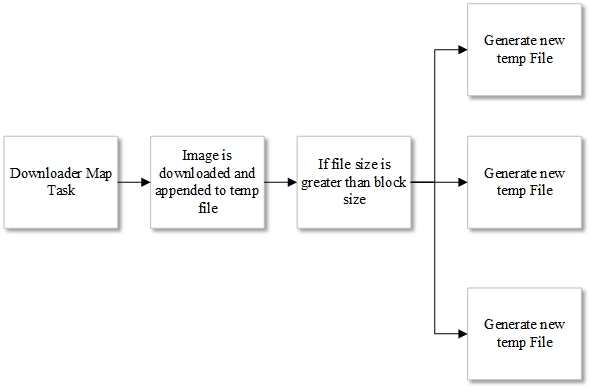
\includegraphics[width=0.45\textwidth]{down-map}
	\caption{Individual map task of Downloader Module}
	\label{fig:down-map}
\end{figure}

\textbf{Step 3: Download image data from URLs.}  For every URL
retrieved in the map task, a connection is established according to
the appropriate transfer protocol (e.g. FTP, HTTP, HTTPS, etc.). Once
connected, we check the file type.  Valid images are assigned
InputStreams associated with the connection. From these InputStreams,
we generate new HImage objects and add the images to the image
bundle. The HImage class holds the image data and provides an
interface for the user's manipulation of image and image header
data. The HImage class also provides interoperability between various
image data types (e.g. BufferedImage, Mat, etc.).

\textbf{ Step 4: Store images in an image bundle. }  Once an HImage
object is received, it can be added to the image bundle simply by
passing the HImage object to the appendImage method. Each map task
generates a number of image bundles depending on the image list. In
the reduce phase, all of these image bundles are merged into one large
bundle.

\begin{figure}[h]
	\centering
	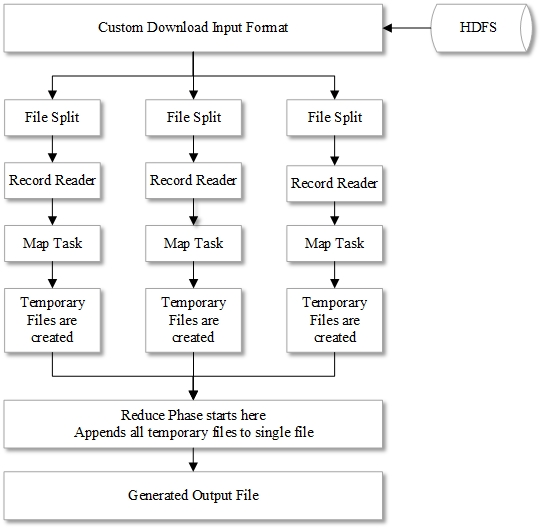
\includegraphics[width=0.45\textwidth]{down-node}
	\caption{Single node running the Downloader Module (handled by
          the framework and transparent to the user)}
	\label{fig:down-node}
\end{figure}

\subsection{Processing image bundle using MapReduce}
Hadoop MapReduce programs handle input and output data very
efficiently, but their native data exchange formats are not convenient
for representing or manipulating image data.  For instance,
distributing images across map nodes require the translation of images
into strings, then later decoding these image strings into specified
formats in order to access pixel information.  This is both
inefficient and inconvenient. To overcome this problem, images should
be represented in as many different formats as possible, increasing
flexibility. The framework focuses on bringing familiar data types
directly to user.

As distribution is important in MapReduce, images should be processed
in the same machine where the bundle block resides. In a generic
MapReduce system, the user is responsible for creating InputFormat and
RecordReader classes to specify the MapReduce job and distribute the
input among nodes. This is a cumbersome and error-prone task; the
Hadoop Image Processing Framework provides such InputFormat and
RecordReaders for the sake of the system's ease of use.

Images are distributed as various image data types and users have
immediate access to pixel values.  If pixel values are naively
extracted from the image byte formats, valuable image header data
(e.g. JPEG EXIF data or IHDR \cite{David03} image headers) is
lost. The framework holds the image data in a special HImageHeader
data type before converting the image bytes into pixel values.  After
processing pixel data, image headers are reattached to the processed
results.  The small amount of storage overhead required for this
functionality is a trade-off worth making for the sake of preserving
image header data after processing.

The functionality of the framework's Processor module is described
below:

\textbf{Step 1: Devise the algorithm.} We assume that the user writes
an algorithm which extends the provided GenericAlgorithm class. This
class is passed as an argument to the processor module. The framework
starts a MapReduce job with the algorithm as an input. The
GenericAlgorithm holds an HImage variable; this allows user to write
an algorithm on a single image data structure, which the framework
then iterates over the entire image bundle. In addition to the
algorithm, the user should provide the image bundle file that needs to
be processed.  Depending on the specifics of the image bundle
organization and contents, the bundle is divided across nodes as
individual map tasks. Each map task will apply the processing
algorithm to each local image and append them in turnto the output
image bundle. In the reduce phase, the Reducer merges these image
bundles into a large image bundle.

\textbf{Step 2: Split image bundle across nodes.} The input image
bundle is stored as blocks in the HDFS.  In order to obtain maximum
throughput, the framework establishes each map task to run in the same
block where it resides, using custom input format and record reader
classes. This allows maximum parallelization without the problem of
transferring data across nodes.  Each image bundle now applies
different map tasks to the image data for which it is responsible.

\begin{figure}[h]
  \centering
  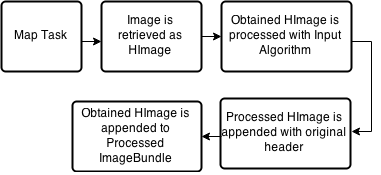
\includegraphics[width=0.45\textwidth]{pro-map}
  \caption{Individual map task of Processor Module}
  \label{fig:pro-map}
\end{figure}

\textbf{Step 3: Process individual image.}  The processing algorithm
devised by the user and provided as input to the Processing Module is
applied to every HImage retrieved in the map task.  The HImage
provides its image data in the data format (e.g. Java BufferedImage,
OpenCV Mat, etc.) requested by the user and used by the processing
algorithm. Once the image data type is retrieved, processing takes
place. After processing, the preserved image header data from the
original image is appended to the processed image. The processed image
is appended to the temporary bundle generated by the map task.

\textbf{Step 4: Store processed images in an image bundle.} Every map
task generates an image bundle upon completion of its processing.
Once the map phase is completed there are many bundles scattered
across the computing cluster.  In the reduce phase, all of these
temporary image bundles are merged into a single large file which
contains all the processed images.

\begin{figure}[h]
  \centering
  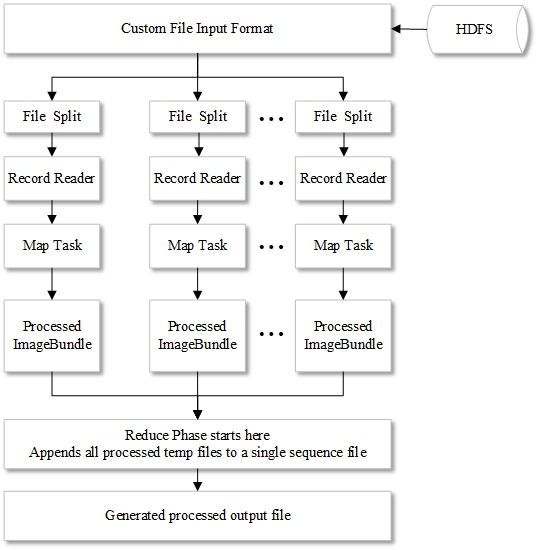
\includegraphics[width=0.45\textwidth]{pro-node}
  \caption{Single node running the Processor Module (handled by
    the framework and transparent to user)}
  \label{fig:pro-node}
\end{figure}

\subsection{Extracting image bundles using MapReduce}
In addition to creating and processing image bundles, the framework
provides a method for extracting and viewing these images.  Generally,
Hadoop extracts images from an image bundle iteratively, inefficiently
using a single node for the task. To address this inefficiency, we
designed an Extractor module which extracts images in parallel across
all available nodes.

Distribution plays a key role in MapReduce; we want to make effective
and efficient use of the nodes in the computing cluster.  As
previously mentioned in the description of the Processor module, a
user working in a generic Hadoop system must again devise custom
InputFormat and RecordReader classes in order to facilitate
distributed image extraction.  The Hadoop Image Processing Framework
provides this functionality for the extraction task as well, providing
much greater ease of use for the development of image processing
applications.

Organizing and specifying the final location of extracted images in a
large distributed task can be confusing and difficult.  Our framework
provides this functionality, and allows the user simply to specify
whether images should be extracted to a local file system or reside on
the Hadoop DFS.
 
The process of the Extractor module is explained below:

\textbf{Step 1: Input the image bundle to be extracted.} The image
bundle specified for extraction is passed as a parameter to the
Extractor module.  In addition, the user can include an optional
parameter specifying the images' final location (defaults to local
file system).  The image bundle is then distributed across the nodes
as individual map tasks. Each map task will extract the requisite
images onto the specified filesystem.

\begin{figure}[h]
  \centering
  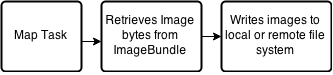
\includegraphics[width=0.45\textwidth]{ext-map}
  \caption{Individual map task of Extractor Module}
  \label{fig:ext-map}
\end{figure}

\textbf{Step 2: Split Image bundle across nodes} The input image
bundle is split across available nodes using the framework's custom
input format and record reader classes for maximum throughput. Once a
map task starts, HImage objects are retrieved.

\textbf{Step 3: Extract individual image} The image bytes obtained
from each HImage object are stored onto the filesystem in the
appropriate file format based on its image type.  The Extractor module
lacks a reduce phase.

\begin{figure}[h]
  \centering
  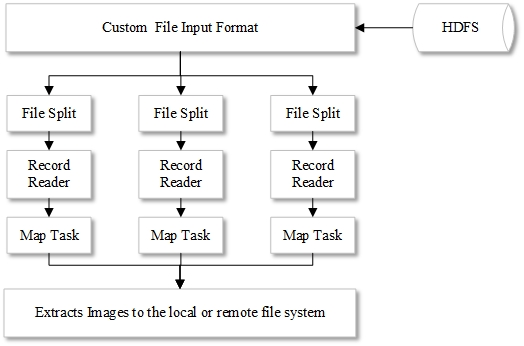
\includegraphics[width=0.45\textwidth]{ext-node}
  \caption{Single node running the Extractor Module (handled by the
    framework and transparent to the user)}
  \label{fig:ext-node}
\end{figure}


\section{Image Processing Computations}
To address the framework capability, we considered to take some existing well used image processing algorihtms and enable running its functionality on a hadoop cluster. These considerations led us to a development of image processing functionality in java for the following computations: flat field correction, canny edge detection and image segmentation. These computations are computationally intensive and data intensive which are operated on range from hundreds to hundred thousands of images. Next we categorize these three computations

%\subsection{Flat Field Correction}
%Flat Field Correction(FFC) is described mathematically below:
%\begin{equation}
%	I^{FFC}(x,y) = \frac{I^{RAW}(x,y)-DI(x,y)}{WI(x,y)-DI(x,y)}
%\end{equation}

%where \begin{math}I^{FFC}(x,y))\end{math} is the flat-field corrected image intensity, \begin{math}DI(x,y)\end{math} is the dark image acquired by closing the camera shutter, \begin{math}I^{RAW}(x,y)\end{math} is the raw uncorrected image density and WI(x,y) is the flat field intensity acquired without any object to correct primarily for spatial shading. This is the simpleset computations that consists of two subtractions and one division for pixel. It needs the DI and WI images co-located from the distributed execution perspective.

\subsection{Laplacian Filter}
The Laplacian is a 2-D isotropic measure of the 2nd spatial derivative of an image. The Laplacian of an image highlights regions of rapid intensity change and is therefore often used for edge detection. The Laplacian is often applied to an image that has first been smoothed with something approximating a Gaussian smoothing filter in order to reduce sensitivity to noise. The operator normally takes a single gray level image as input and produces another gray level image as output.

The Laplacian \begin{math} L(x,y)\end{math}of an image with pixel intensity values \begin{math}I(x,y)\end{math} is given by 
\begin{equation}
L(x,y) = \frac{\partial^2 I}{\partial x^2} + \frac{\partial^2 I}{\partial y^2}
\end{equation} 

This is calculated using a convolution filter.

Since the input image is represented as a set of discrete pixels, we have to find a discrete convolution kernel that can approximate the second derivatives in the definition of the Laplacian. This a simplest computation that consists of few additions and multiplications.

\subsection{Canny Edge Detection}
Canny Edge Detection\cite{Canny86} is an multi-stage algorithm to detect a wide range of edges in images. Edge detection, especially step edge detection is an important technique to extract useful structural information from different vision objects and dramatically reduce the amount of data to be processed. Among the edge detection methods developed so far, canny edge detection algorithm is one of the most strictly defined methods that provides good and reliable detection.

The process of Canny edge detection algorithm can be broken down to 5 different stages:

\begin{itemize}
	\item Apply Gaussian filter to smooth the image in order to remove the noise.
	\item Find the intensity gradients of the image.
	\item Apply non-maximum suppression to get rid of spurious response to edge detection
	\item Apply double threshold to determine potential edges.
	\item Track edge by hysteresis. Finalize the detection of edges by suppressing all the other edges that are weak and not connected to strong edges. 
\end{itemize}


\subsection{Image segmentation using k-means clustering}
K-Means algorithm is an unsupervised clustering algorithm that classifies the input data points into multiple classes based on their inherent distance from each other. The algorithm assumes that the data features form a vector space and tries to find natural clustering in them. The points are clustered around centroids \begin{math}\mu_{i} \forall i = 1...k\end{math} which are obtained by minimizing the objective
\begin{equation}
	V = \sum\limits_{i=1}^n \sum\limits_{x_{j}\in S_{i}} (x_{j} - \mu_{i})^2
\end{equation}

where there are \begin{math}k\end{math} clusters \begin{math} S_{i},i=1,2,...,k \end{math} and \begin{math} \mu_{i} \end{math} is the centroid or mean point of all the points \begin{math}x_{j} \in S_{i}\end{math} 

As a part of the experiment, an iterative version of the algorithm was implemented. The algorithm takes a 2 dimensional image as input. Various steps in the algorithm are as follows:

\begin{itemize}
	\item Compute the intensity distribution(also called the histogram) of the intensities.
	\item Initialize the centroids with k random intensities.
	\item Repeat the following steps until the cluster labels of the image does not change anymore.
	\item Cluster the points based on distance of their intensities from the centroid intensities.
	\begin{equation}
		c^{i} := arg min_{j}||x^{i} - \mu_{j}||^2
	\end{equation}
	\item Compute the new centroid for each of the clusters.
	\begin{equation}
		\mu_{i} = \frac{\sum\limits_{i=1}^{m} 1\{c_{i} = j\}x^i}{\sum\limits_{i=1}^{m} 1\{c_{i} = j\}}
	\end{equation}
	
	where \begin{math}k\end{math} is a parameter of the algorithm (the number of clusters to be found), \begin{math}i\end{math} iterates over that all the intensities, \begin{math}j\end{math} iterates over all the centroids and \begin{math}\mu_{i}\end{math} are the centroid intensities.
\end{itemize}
	

\section{Experimental Results}


We describe two image processing algorithms using Hadoop Image Processing framework. These image processing algorithms are relatively simple to implement on a single node, implementing these algorithms are complex and inefficient on existing platforms, yet simple to implement using the framework.In the following section we provided image processing computations with the data set described in Section VA. The hardware and software specifications are provided in Section VB as well as observations in Section VC 


%\begin{figure}[h]
%	\centering
%	
\includegraphics[width=0.45\textwidth]{input-canny}
%	\caption{A Sample Image from downloaded image bundle}
%	\label{fig:input-canny}
%\end{figure}

%\begin{figure}[h]
%	\centering
%	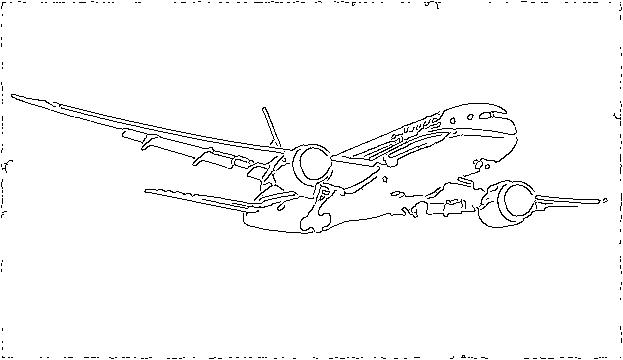
\includegraphics[width=0.45\textwidth]{output-canny}
%	\caption{Processed image using canny edge detection}
%	\label{fig:output-canny}
%\end{figure}

\subsection{Characteristics of Image Dataset, Hardware and Software}
We computed image processing computations on a dataset which is about 1TB size. The data set is made from the flickr search based on a keyword flight. The data set is extracted using the a FlickrRipper in the framework which implements Ripper Interface. The Ripper interface can be implemented for any custom Rippers to get the image URLs. The example data set is composed of 220000 images at 4.76 MB/image equals to 1 TB.  

\subsection{Computer Hardware and Software Characterstics}
We ran the image processing computations on a cluster with 6 nodes and on a desktop computer. Table summarizes the cluster and desktop hardware and software specifications. The cluster nodes differ in terms of CPU speed and RAM. We installed hadoop, cloudera CDH5 and java 1.7 on the cluster to support java code execution. The desktop computer had similar software configuration to the cluster.

\begin{table}[h]
	\begin{tabular}{|l|l|l|l|}
		\hline
		& \multicolumn{1}{c|}{\textbf{Specs}}                            & \multicolumn{1}{c|}{\textbf{Cluster}}                                                                                                           & \multicolumn{1}{c|}{\textbf{Desktop}}                                                                               \\ \hline
		\multirow{2}{*}{Hardware} & Cluster Nodes                                                  & \begin{tabular}[c]{@{}l@{}}6 datanodes having \\ from 2 to 4 virtual \\ processors with 4 GB\\ RAM and namenode \\ having 8 GB RAM\end{tabular} & \begin{tabular}[c]{@{}l@{}}Intel Xeon @ 2Ghz\\ 8 cores, 16GB of RAM \\ and hyper threading\\ activated\end{tabular} \\ \cline{2-4} 
		& Networking                                                     & 1Gbit/second                                                                                                                                    &                                                                                                                     \\ \hline
		\multirow{3}{*}{Software} & \begin{tabular}[c]{@{}l@{}}Java Virtual\\ Machine\end{tabular} & \begin{tabular}[c]{@{}l@{}}Java version \\ "1.7.0\_45"\\ Java SE Runtime\\ Environment\end{tabular}                                             & \begin{tabular}[c]{@{}l@{}}Java version \\ "1.7.0\_45"\\ Java SE Runtime\\ Environment\end{tabular}                 \\ \cline{2-4} 
		& Hadoop                                                         & \begin{tabular}[c]{@{}l@{}}hadoop 2.5\\ cloudera CDH5\end{tabular}                                                                              &                                                                                                                     \\ \cline{2-4} 
		& \begin{tabular}[c]{@{}l@{}}Operating\\ System\end{tabular}     & CentOS 6.5                                                                                                                                      & CentOS 6.5                                                                                                          \\ \hline
	\end{tabular}
\end{table}


\subsection{Observations}   

The desktop implementation of the Algorithm is a java program for processing a small image dataset. As soon as the data set is processed the program halts. The desktop implementation starts as a single thread. One image is processed every time. As soon as the image is processed, it starts processing a new image. When the data set size is low, the program runs smooth with best performance. As data set size increases to Tera-bytes the system can't handle such huge amounts of data. To handle such large amounts of data we use the distributed computing using hadoop.



\begin{figure}[h]
	\centering
	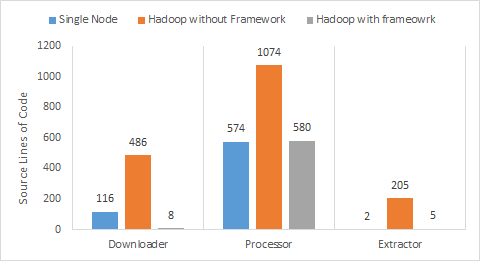
\includegraphics[width=0.45\textwidth]{module-chart}
	\caption{Module Chart}
	\label{fig:module-chart}
\end{figure}
 

The Algorithm is implemented on a hadoop cluster without using framework. It overcomes the problem of handling large datasets but suffers with a problem of code complexity. The user needs to write a huge amount of code and understand the technical details of hadoop. Writing such huge amounts of code including the custom InputFormats and RecordReaders is cumbersome. Fig.\ref{fig:module-chart} compares the actual lines of code user needs to write to run an Image Processing application in hadoop cluster which makes an average user life harder to use the hadoop features.

The Algorithm is finally implemented on a hadoop cluster using the framework. It overcomes many problems handling large datasets, code complexity, interoperability between image datatypes etc., The process of creating CustomInputFormat and RecordReader is automated as per the input. User can tune the settings using different getter and setter method to get the desired output. The framework is so transparent that the user needs to input few lines of code to process a large image data set. It hides all the MapReduce Technical details and runs the code highly parallelized. The key differences among the three platform-specific implementation lie in computation elasticity and code complexity associated with each platform.


\begin{table}[h]
	\begin{tabular}{|l|l|l|l|}
		\hline
		\multicolumn{1}{|c|}{\textbf{\begin{tabular}[c]{@{}c@{}}Computa-\\ tional\\ Platform\end{tabular}}} & \multicolumn{1}{c|}{\textbf{\begin{tabular}[c]{@{}c@{}}Computational \\ Elasticity\end{tabular}}}      & \multicolumn{1}{c|}{\textbf{\begin{tabular}[c]{@{}c@{}}Code \\ Complexity\end{tabular}}}                                                                                                                                                  & \multicolumn{1}{c|}{\textbf{\begin{tabular}[c]{@{}c@{}}Data \\ Locality\end{tabular}}}                                                                           \\ \hline
		Desktop                                                                                             & \begin{tabular}[c]{@{}l@{}}Low : limited by \\ RAM and CPU of \\ the executing\\ computer\end{tabular} & \begin{tabular}[c]{@{}l@{}}Normal : Complexity \\ lies in writing the \\ algorithm\end{tabular}                                                                                                                                           & \begin{tabular}[c]{@{}l@{}}All data are \\ on local disk\end{tabular}                                                                                            \\ \hline
		\begin{tabular}[c]{@{}l@{}}Hadoop:\\ without \\ using \\ framework\end{tabular}                     & \begin{tabular}[c]{@{}l@{}}High: Nodes can\\  be requested \\ as needed\end{tabular}                   & \begin{tabular}[c]{@{}l@{}}Heavy : Complexity \\ lies inwriting every \\ module in framework \\ including custom \\ Input Formats and \\ RecordReaders.User \\ should have high \\ technical knowledge on \\ hadoop working.\end{tabular} & \begin{tabular}[c]{@{}l@{}}All data resides\\ in HDFS. Custom\\ InputFormats \\ needsto be \\ created to launch\\ computations \\ where thedata are\end{tabular} \\ \hline
		\begin{tabular}[c]{@{}l@{}}Hadoop:\\ using \\ framework\end{tabular}                                & \begin{tabular}[c]{@{}l@{}}High: Nodes can \\ be requested \\ as needed\end{tabular}                   & \begin{tabular}[c]{@{}l@{}}Normal : Complexity \\ lies in writing \\ algorithm and is \\ equivalent to writing \\ in Desktop platform\end{tabular}                                                                                        & \begin{tabular}[c]{@{}l@{}}All data resides \\ in HDFS. Highly \\ parallelized.\end{tabular}                                                                     \\ \hline
	\end{tabular}
\end{table}



   
\iffalse
\begin{table}[h]
	\centering
	\begin{tabular}{|c|c|c|}
		\hline
		\textbf{Module} & \textbf{\begin{tabular}[c]{@{}c@{}}SLOC \\ using framework\end{tabular}}                                                          & \textbf{\begin{tabular}[c]{@{}c@{}}SLOC \\ without framework\end{tabular}}                                                                                    \\ \hline
		Downloader      & 3 - 5 lines                                                                                                                       & \begin{tabular}[c]{@{}c@{}}300 - 1000 lines.\\ Custom Input Formats\\ and RecordReaders are\\ to be implemented\end{tabular}                                  \\ \hline
		Processor       & 3 - 5 lines                                                                                                                       & \begin{tabular}[c]{@{}c@{}}400 - 1000 lines\\ Many overheads. \\ Converting to image \\ data types, Mapper \\ locality should be taken\\ care of\end{tabular} \\ \hline
		Extractor       & 2 - 8 lines                                                                                                                       & \begin{tabular}[c]{@{}c@{}}200 - 1000 lines\\ Depends on the extraction\\ process.\end{tabular}                                                               \\ \hline
		Algorithm       & \begin{tabular}[c]{@{}c@{}}200 - 300 lines\\ adds a few lines overhead\\ to automate the process\\ for MapReduce job\end{tabular} & 200 - 250 lines                                                                                                                                               \\ \hline
	\end{tabular}
\end{table}
\fi


Hadoop Image processing framework provides transparency over two levels. The first level of transparency allows user to use the predefined MapReduce modules Downloader, Processor and Extractor for processing the image modules. The second of level of transparency allows the users to write custom map reduce programs as the framework is built in an hierarchal manner.

The great thing about Hadoop Image Processing framework is its built in such a way that using it is really simple. The framework strictly adheres java file writing and reading techniques and extends it to a new level of BundleFile Writing and Reading using hadoop framework. This makes user to work with hadoop image processing more flexible and easier. The main aim of the framework is to provide an abstractness in such a way that programming on a single computer is equivalent to programming on a hadoop cluster.  Listing 1. provides the similarities in code writing in java and image processing framework. Making framework similar to java helps understanding the framework more easier and reduces complexity.


\begin{figure}[h]
	\centering
	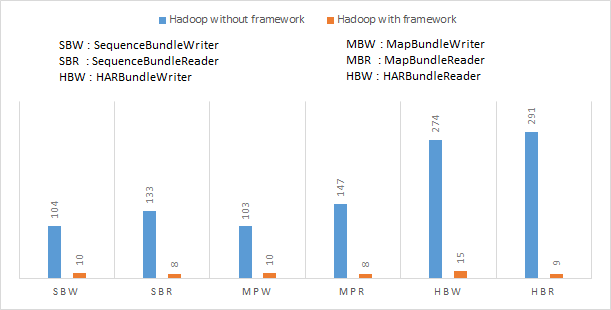
\includegraphics[width=0.45\textwidth]{files-chart}
	\caption{Comparing File Writers and readers without and with using framework }
	\label{fig:files-chart}
\end{figure}

\begin{lstlisting}[caption = Comparing File Writer instance in java and SequenceBundleWriter instance in Hadoop Image Processing framework ]

//Sample File Writing in Java

File file = new File("abc.txt");
FileWriter fw=new FileWriter(file);
fw.append(val)
fw.close();

//Sample BundleFile Writing in Hadoop using Framework

BundleFile file = new BundleFile("abc.seq");
SequenceBundleWriter sbw=new SequenceBundleWriter(file);
sbw.append(himage);
sbw.close();

\end{lstlisting}


\section{Conclusion}
This paper has described our framework fo image processing for large scale image processing applications on the MapReduce framework. The framework is designed to abstract the technical details of Hadoop's powerful MapReduce framework and provide a way for users who want to process large image datasets. We provided a how the images can be stored in different hadoop file format and efficient access within Map Reduce pipeline and simple modules to make the framework more easier. By providing interoperability between different image data types we give the user to process the images using different open-source image processing libraries. Finally, we provide a way to overcome the loss of image headers after processing which are most useful for image processing and vision applications.

With these features, the framework brings a new level of transparency and simplicity for creating large-scale image processing applications over Hadoop's MapReduce framework. The paper describes to example applications built using the framework to demonstrate the power of the framework. We hope that this level of abstractness to use Hadoop MapReduce framework will enhance the ability to create large-scale image processing applications with ease.

\section{Future Work}
In the near future we hope to extend the framework into a full-fledged multimedia processing framework. We would like to improve framework such that audio and video processing over hadoop is done with ease. We also intend to add a CUDA module for using the graphics card for processing the images. Finally, we intend to wrap our system into an highly parallelized open-source hadoop multimedia processing framework and perhaps provide a sample web-based graphic user interface with all image processing applications.  

	\bibliography{references}
	\bibliographystyle{IEEEtran}

\end{document}

